\documentclass[svgnames,tikz]{standalone}
\usetikzlibrary{3d}

\begin{document}
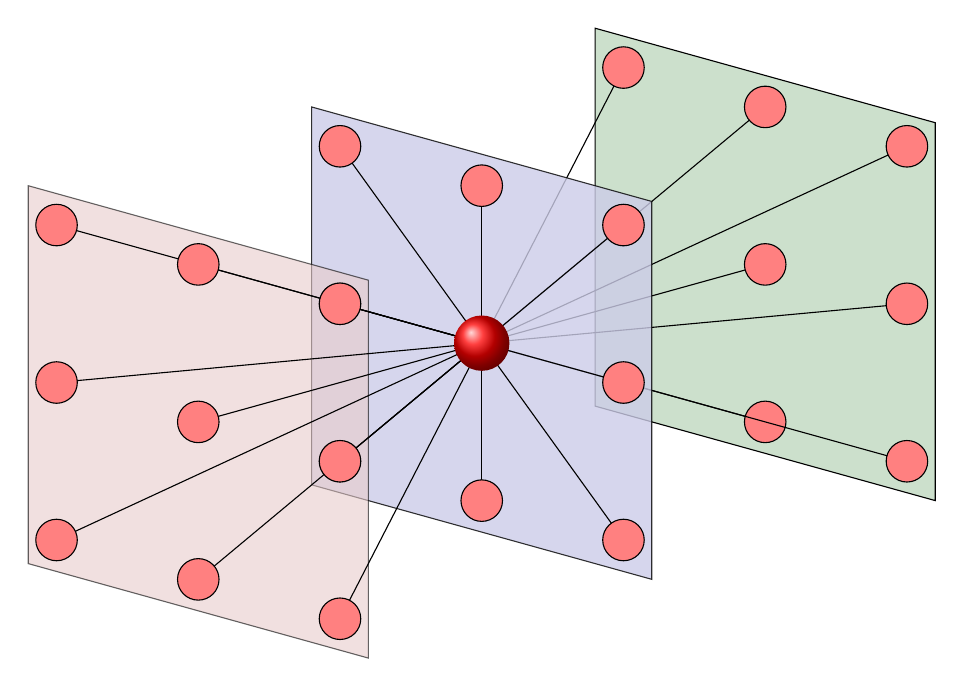
\begin{tikzpicture}[scale=2,x={(0.9,-0.25)},z={(2,1)}]
  \tikzset{ nbh/.style={draw, circle, fill=red!50, minimum width=15pt} };


  \node[circle, inner sep=5pt] (A) {};

  \begin{scope}[canvas is yx plane at z=1]
    \draw[fill=DarkGreen!20,opacity=1] (-1.2,-1.2) rectangle (1.2,1.2);
  \end{scope}

  \foreach \j in {-1,0,1}
  \foreach \k in {-1,0,1}
  \draw (A) -- (\j,\k,1) node[nbh] {};


  \begin{scope}[canvas is yx plane at z=0]
    \draw[fill=DarkBlue!20,opacity=0.8] (-1.2,-1.2) rectangle (1.2,1.2);
  \end{scope}




  \foreach \j in {-1,0,1}
  \foreach \k in {-1,0,1}
  {
    \if\j\k
    \if0\j
    \else
    \draw (A) -- (\j,\k,0) node[nbh] {};
    \fi
    \else
    \draw (A) -- (\j,\k,0) node[nbh] {};
    \fi
  }

  \begin{scope}[canvas is yx plane at z=-1]
    \draw[fill=DarkRed!20,opacity=0.6] (-1.2,-1.2) rectangle (1.2,1.2);
  \end{scope}

  \foreach \j in {-1,0,1}
  \foreach \k in {-1,0,1}
  \draw (A) -- (\j,\k,-1) node[nbh] {};

  \shade[ball color = red] (0,0) circle (5pt);
  \end{tikzpicture}
\end{document}
